\subsection{Example: Slider-crank Mechanism}
\begin{frame}{Normal Approach}
	\begin{block}{Example 1: Slider-crank Mechanism}
		\begin{table}
			\begin{minipage}{0.5\linewidth}
				\begin{tabular}{l|l}
					& $l_{AB}=l_1=0.5m$ \\
					& $l_{BC}=l_2=1m$ \\
					Given& $\theta_1=60^\circ$ \\
					& $\vb{\omega}{1} = 1\kh $ $(rad/s)$\\
					& $\vb{\alpha}{1} = -1\kh $ $(rad/s^2)$ \\\hline
					Find & $\vb{v}{B}$, $\vb{v}{C}$, $\vb{a}{B}$, $\vb{a}{C}$,\\
					 &\boldmath{$\vb{\omega}{2}$}, \boldmath{$\vb{\alpha}{2}$}\\
				\end{tabular}
			\end{minipage}\hfill
			\begin{minipage}{0.5\linewidth}
				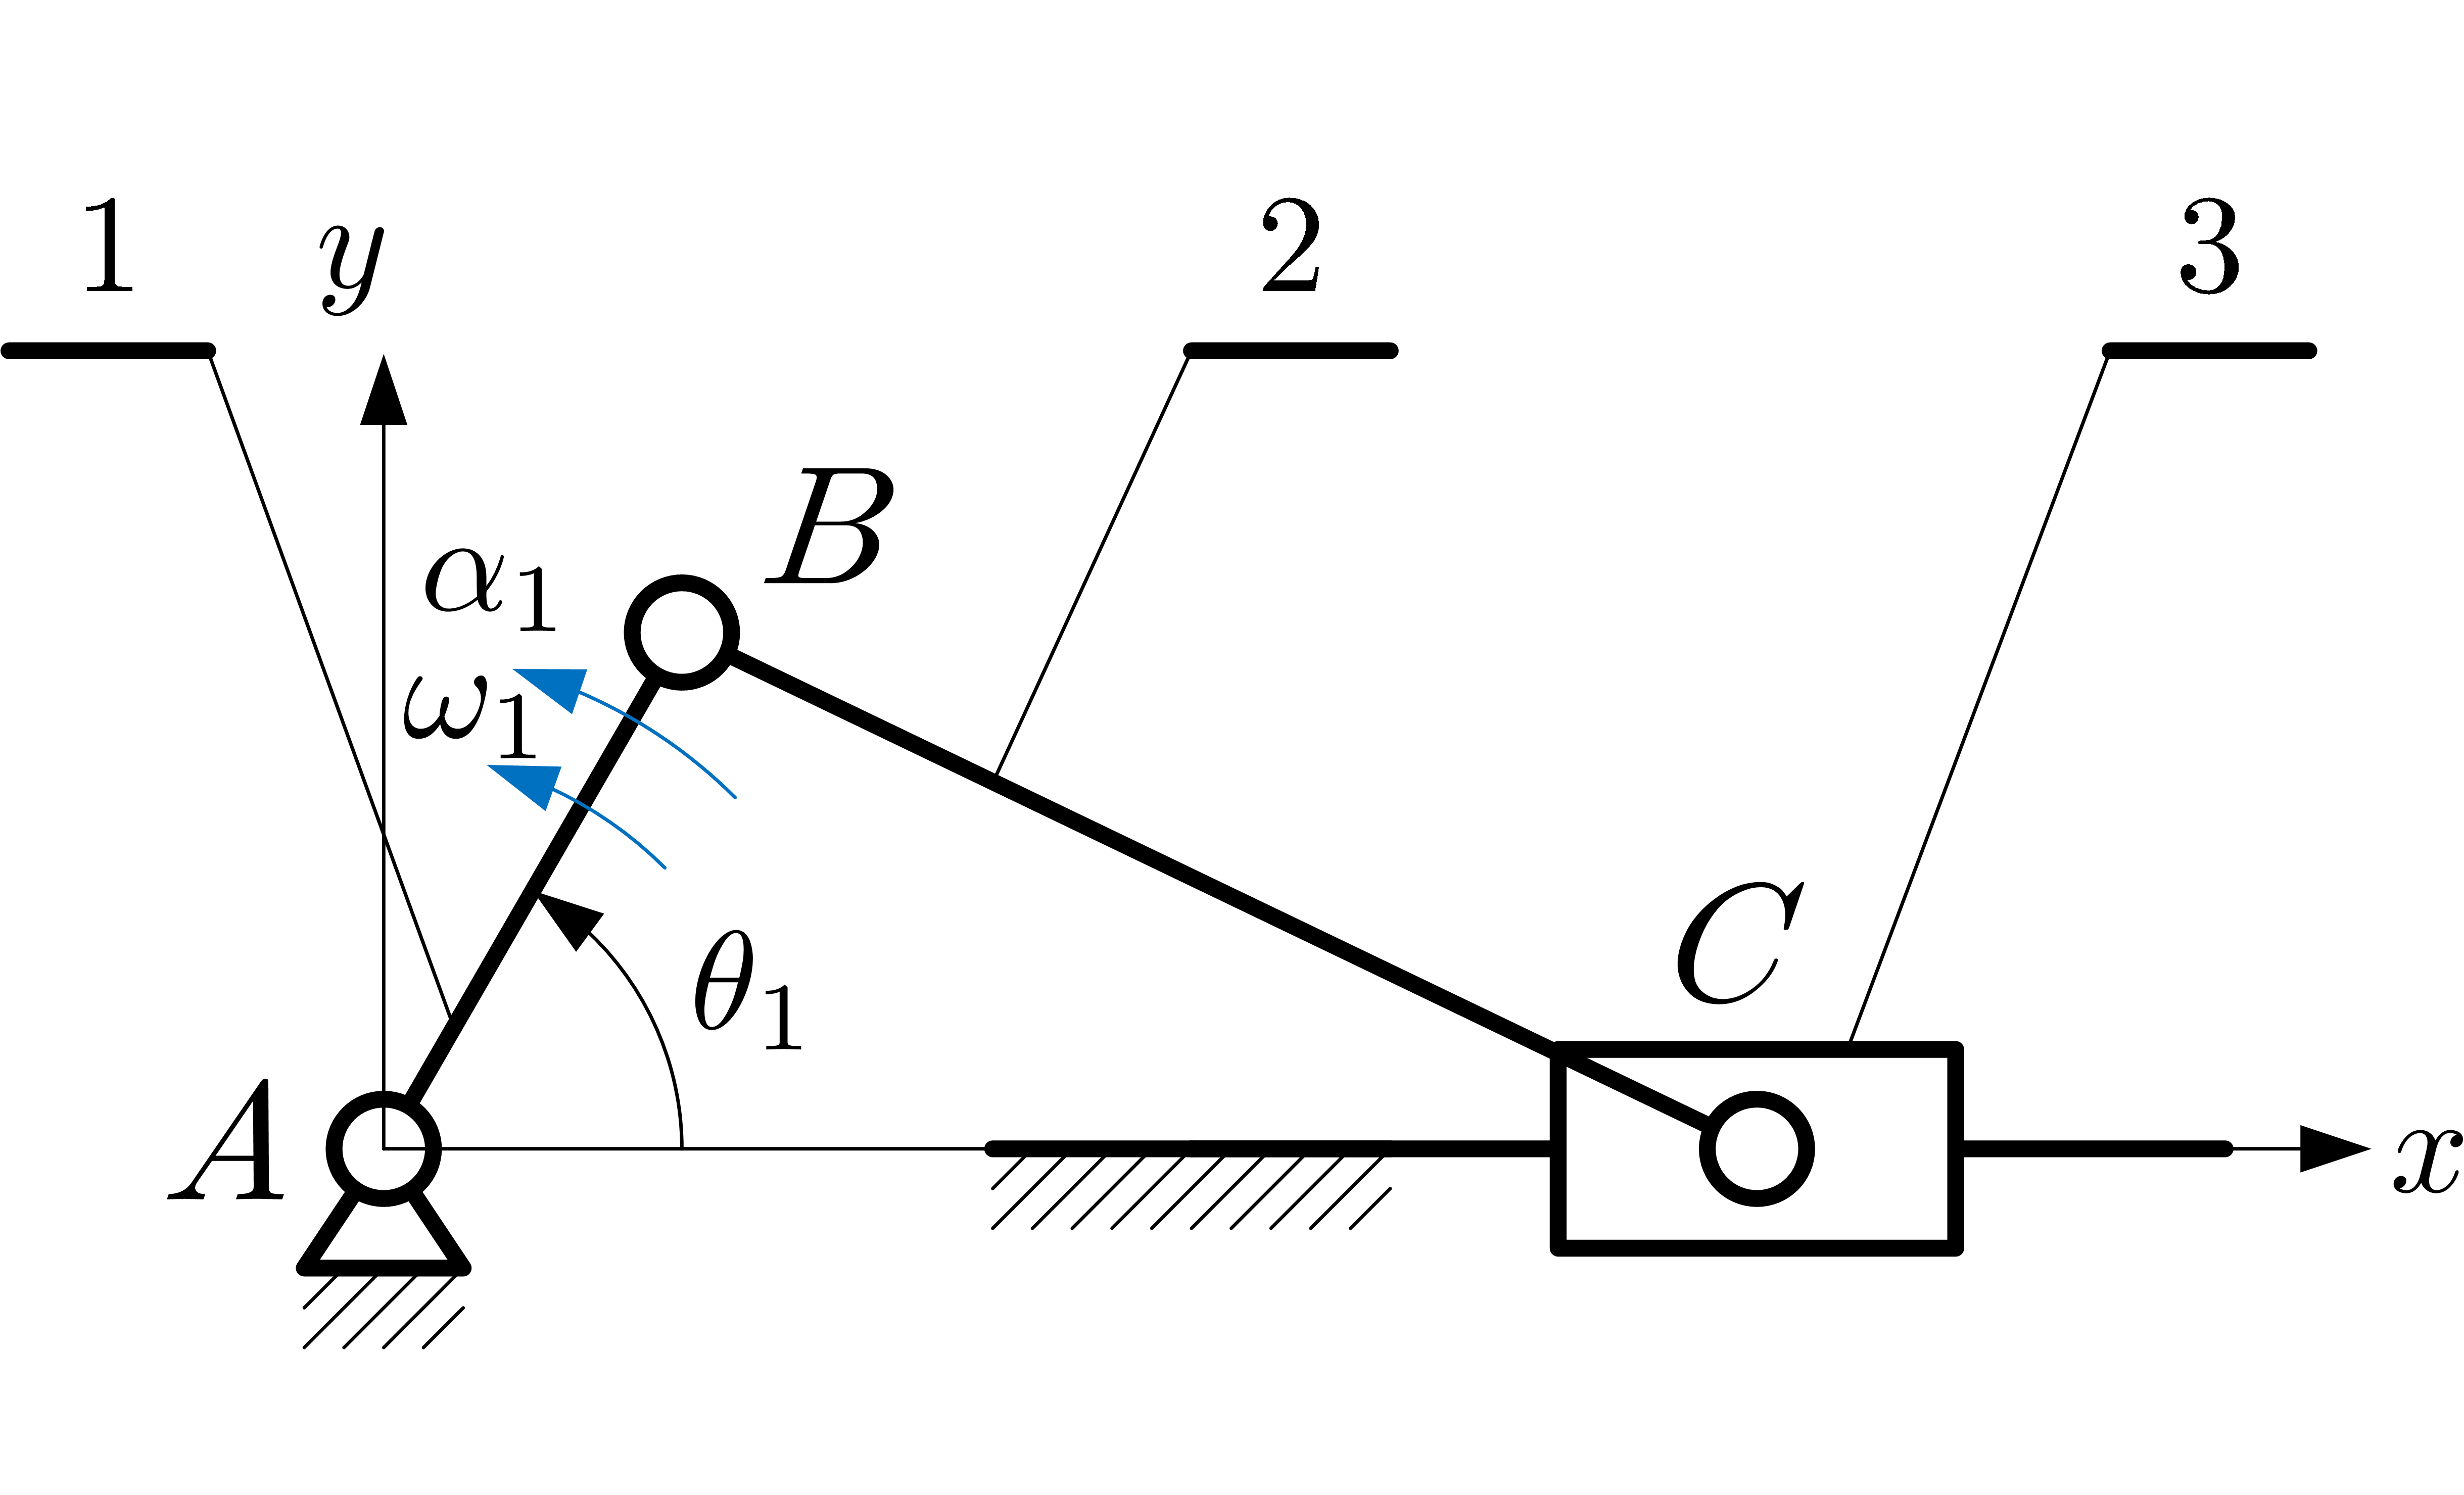
\includegraphics[width=50mm]{images/R-RRT.png}
			\end{minipage}
		\end{table}
	\end{block}
\emph{Solution}\vskip2.5mm
Using position analysis / MATLAB,\vskip1.25mm
$\Rightarrow \vb{r}{B} = 0.25\ih + 0.433\jh\text{ $(m)$}, \vb{r}{C} = 1.1514\ih \text{ $(m)$}$\\
$\vb{r}{CB} = \vb{r}{C}-\vb{r}{B}=0.9014\ih-0.433\jh \text{ $(m)$}$
\end{frame}

\begin{frame}
\begin{itemize}
	\item Find $\vb{v}{B}$\vskip1.25mm
	$\vb{v}{B} = \vb{\omega}{1} \times \vb{r}{B} = -0.433\ih + 0.25\jh \text{ $(m/s)$}$\vskip2.5mm
	\item Find $\vb{v}{C}$, $\vb{\omega}{2}$\vskip1.25mm
	$\vb{v}{C} = \vb{v}{B} + \vb{v}{CB} = \vb{v}{B} + \vb{\omega}{2}\times \vb{r}{CB}$\vskip2.5mm
%	$v_{Cx}\ih = (-0.433\ih + 0.25\jh) + \omega_{2z}\kh\times(0.9014\ih-0.433\jh)$\vskip2.5mm
	Projecting onto $x,y$-axes, we obtain the solution:\vskip1.25mm
	$\Rightarrow\begin{cases}
	v_{Cx} = -0.5531\text{ $(m/s)$}\\ \omega_{2z}=-0.2774\text{ $(rad/s)$}
	\end{cases}$\\$\Rightarrow\begin{cases}
	\vb{v}{C} = -0.5531\ih\text{ $(m/s)$}\\ \vb{\omega}{2}=-0.2774\kh\text{ $(rad/s)$}
	\end{cases}$
\end{itemize}
\end{frame}
\begin{frame}
	\begin{itemize}
		\item Find $\vb{a}{B}$, $\vb{a}{^n_{CB}}$
		\vskip1.25mm
		$\vb{a}{B} = \vb{\alpha}{1}\times \vb{r}{B} - \vb{\omega}{1}^2\vb{r}{B}=0.183\ih - 0.683\jh \text{ $(m/s^2)$}$\\
		$\vb{a}{^n_{CB}}=- \vb{\omega}{2}^2\vb{r}{CB}=-0.0693\ih+0.0333\jh\text{ }(m/s^2)$
		\vskip2.5mm
		\item Find $\vb{a}{C}$, $\vb{\alpha}{2}$
		\vskip1.25mm
		$\vb{a}{C} = \vb{a}{B} + \vb{a}{CB} = \vb{a}{B} + \vb{\alpha}{2}\times \vb{r}{CB} - \vb{\omega}{2}^2\vb{r}{CB}$
%		$a_{Cx}\ih = 0.1137\ih-0.6497\jh+ \alpha_{2z}\kh\times(0.9014\ih-0.433\jh)$
		\vskip2.5mm
		Projecting onto $x,y$-axes, we obtain the solution:
		\vskip1.25mm
		$\Rightarrow\begin{cases}
			a_{Cx} = 0.4258\text{ $(m/s^2)$}\\\alpha_{2z}=0.7208\text{ }(rad/s^2)
		\end{cases}$\\
		$\Rightarrow\begin{cases}
		\vb{a}{C} = 0.4258\ih\text{ $(m/s^2)$}\\\vb{\alpha}{2}=0.7208\kh\text{ }(rad/s^2)
		\end{cases}$\\
	\end{itemize}
\end{frame}
\begin{frame}{MATLAB R2019a code}
\lstinputlisting[style=Matlab-editor, basicstyle=\mlttfamily]{codes/s-c_v.m}
\end{frame}
\begin{frame}{MATLAB R2019a code}
\lstinputlisting[style=Matlab-editor, basicstyle=\mlttfamily]{codes/s-c_a.m}
\end{frame}

\begin{frame}{Derivative Method}
	Let $\theta_1=\theta(t)$ be a function of time $t$. We perform position analysis to find $\vb{r}{B}(\theta(t))$ and $\vb{r}{C}(\theta(t))$. Using MATLAB, we find out that:\vskip1.25mm
	\hskip20mm$\displaystyle \vb{r}{B}(\theta(t)) = \frac{\cos{\theta(t)}}{2}\ih + \frac{\sin{\theta(t)}}{2}\jh$\vskip1.25mm
	\hskip20mm$\displaystyle \vb{r}{C}(\theta(t)) = \left(\frac{cos{\theta(t)}}{2} + \frac{\sqrt{2 - \sin{\theta(t)}}\sqrt{\sin{\theta(\theta(t))} + 2)}}{2}\right)\ih$\vskip2.5mm
	Using the results above to obtain the angle  $\theta_2(\theta(t))$ of link 2:
	\[\displaystyle\theta_2(\theta(t))=\arctan{\left(-\frac{\sin{\theta(t)}}{\sqrt{2 - \sin{\theta(t))}}\sqrt{\sin{\theta(t)} + 2}}\right)}\]
\end{frame}
\begin{frame}
Then, find velocities and accelerations by taking first and second derivative of $\vb{r}{B}$, $\vb{r}{C}$, $\theta_2$, respectively:
\[\begin{cases}
\displaystyle \vb{v}{B}(\theta(t))=\xvec[.]{\bm{r}}_{\bm{B}}\\\displaystyle \vb{v}{C}(\theta(t))=\xvec[.]{\bm{r}}_{\bm{C}}\\\displaystyle \vb{\omega}{2}(\theta(t))=\dot{\theta_2}\kh
\end{cases}, \begin{cases}
\displaystyle \vb{a}{B}(\theta(t))=\xvec[:]{\bm{r}}_{\bm{B}}\\\displaystyle \vb{a}{C}(\theta(t))=\xvec[:]{\bm{r}}_{\bm{B}}\\\displaystyle \vb{\alpha}{2}(\theta(t))=\ddot{\theta_2}\kh
\end{cases}\]
Let $\theta(t)=60^\circ$, we obtain the final results.
\end{frame}
\begin{frame}{MATLAB R2019a code}
	\lstinputlisting[style=Matlab-editor, basicstyle=\mlttfamily]{codes/s-c_p_d.m}
\end{frame}
\begin{frame}{MATLAB R2019a code}
\lstinputlisting[style=Matlab-editor, basicstyle=\mlttfamily]{codes/s-c_v_a_d.m}
\end{frame}
\begin{frame}{Independent Contour Method}
	Using the solution above,\vskip1.25mm
	$\vb{r}{B} = 0.25\ih + 0.433\jh\text{ $(m)$}, \vb{r}{C} = 1.1514\ih \text{ $(m)$}$ \\
	$\vb{r}{CB}=0.9014\ih-0.433\jh \text{ $(m)$}$, $ \vb{a}{B}=0.183\ih - 0.683\jh \text{ $(m/s^2)$}$\vskip2.5mm
	Applying velocity formulas to find $\vb{\omega}{12} = \omega_{12z}\kh$, $\vb{\omega}{23} = \omega_{23z}\kh$,
	$\vb{v}{23} = v_{23x}\ih\kh$:
	\vskip1.25mm% and notice that there exists $\vb{v}{23}$ corresponding to slider 2:\vskip1.25mm
	$\begin{cases}
	\vb{\omega}{01} + \vb{\omega}{12} + \vb{\omega}{23} = \vb{0}{}\\
	\vb{r}{B}\times\vb{\omega}{12} + \vb{r}{C}\times\vb{\omega}{23} + \vb{v}{23} = \vb{0}{}
	\end{cases}$\vskip2.5mm%\$\Rightarrow\begin{cases}
%	1\kh+\omega_{12z}\kh + \omega_{23z}\kh=\vb{0}{}\\
%	(0.25\ih + 0.433\jh)\times\omega_{12z}\kh+(1.1514\ih)\times\omega_{23z}\kh+v_{23x}\ih=\vb{0}{}
%	\end{cases}$\vskip2.5mm
	Solving the system of equations by projecting onto $x,y$-axes, we obtain:\vskip1.25mm $\text{\boldmath$\vb{\omega}{12}$}=-1.2774\kh\text{ }(rad/s)$, $\text{\boldmath$\vb{\omega}{23}$}=0.2774\kh\text{ }(rad/s)$,
	$\vb{v}{23}=0.5531\ih\text{ }(m/s)$\vskip2.5mm
	The results is consistent with the 2 previous methods.
\end{frame}

\begin{frame}
	Again, using acceleration formulas and notice that there exists $\vb{a}{23}$ corresponding to slider 2:\vskip1.25mm
	$\begin{cases}
	\text{\boldmath$\vb{\alpha}{01}$}+\text{\boldmath$\vb{\alpha}{12}$}+\text{\boldmath$\vb{\alpha}{23}$}=\vb{0}{}\\
	\vb{r}{B}\times\text{\boldmath$\vb{\alpha}{12}$}+\vb{r}{C}\times\text{\boldmath$\vb{\alpha}{23}$}+\vb{a}{23}-\vb{\omega}{1}^2\vb{r}{B}-\vb{\omega}{2}^2\vb{r}{CB}=\vb{0}{}
	\end{cases}$\vskip2.5mm%\\$\Rightarrow\begin{cases}
%	-1\kh+\alpha_{12z}\kh + \alpha_{23z}\kh=\vb{0}{}\\
%	(0.25\ih + 0.433\jh)\times\alpha_{12z}\kh+(1.1514\ih)\times\alpha_{23z}\kh+a_{23x}\ih\\\hskip40mm-0.3193\ih-0.3997\jh=\vb{0}{}
%	\end{cases}$\vskip2.5mm
	Solving the system of equations by projecting onto $x,y$-axes, we obtain:\vskip1.25mm $\text{\boldmath$\vb{\alpha}{12}$}=1.7208\kh\text{ }(rad/s^2)$, $\text{\boldmath$\vb{\alpha}{23}$}=-0.7208\kh\text{ }(rad/s^2)$,
	$\vb{a}{23}=-0.4258\ih\text{ }(m/s^2)$\vskip2.5mm
	The results is consistent with the 2 previous methods.
\end{frame}
\begin{frame}{MATLAB R2019a code}
\lstinputlisting[style=Matlab-editor, basicstyle=\mlttfamily]{codes/s-c_v_i.m}
\end{frame}
\begin{frame}{MATLAB R2019a code}
\lstinputlisting[style=Matlab-editor, basicstyle=\mlttfamily]{codes/s-c_v_i_2.m}
\end{frame}
\begin{frame}{MATLAB R2019a code}
\lstinputlisting[style=Matlab-editor, basicstyle=\mlttfamily]{codes/s-c_a_i.m}
\end{frame}
\begin{frame}{MATLAB R2019a code}
\lstinputlisting[style=Matlab-editor, basicstyle=\mlttfamily]{codes/s-c_a_i_2.m}
\end{frame}
\begin{frame}{Velocity - Acceleration plotting}
\lstinputlisting[style=Matlab-editor, basicstyle=\mlttfamily]{codes/s-c_v_a_plotting.m}
\end{frame}
\begin{frame}{Output figures}
\begin{table}
\begin{minipage}{0.5\linewidth}
	\begin{figure}
		\centering
		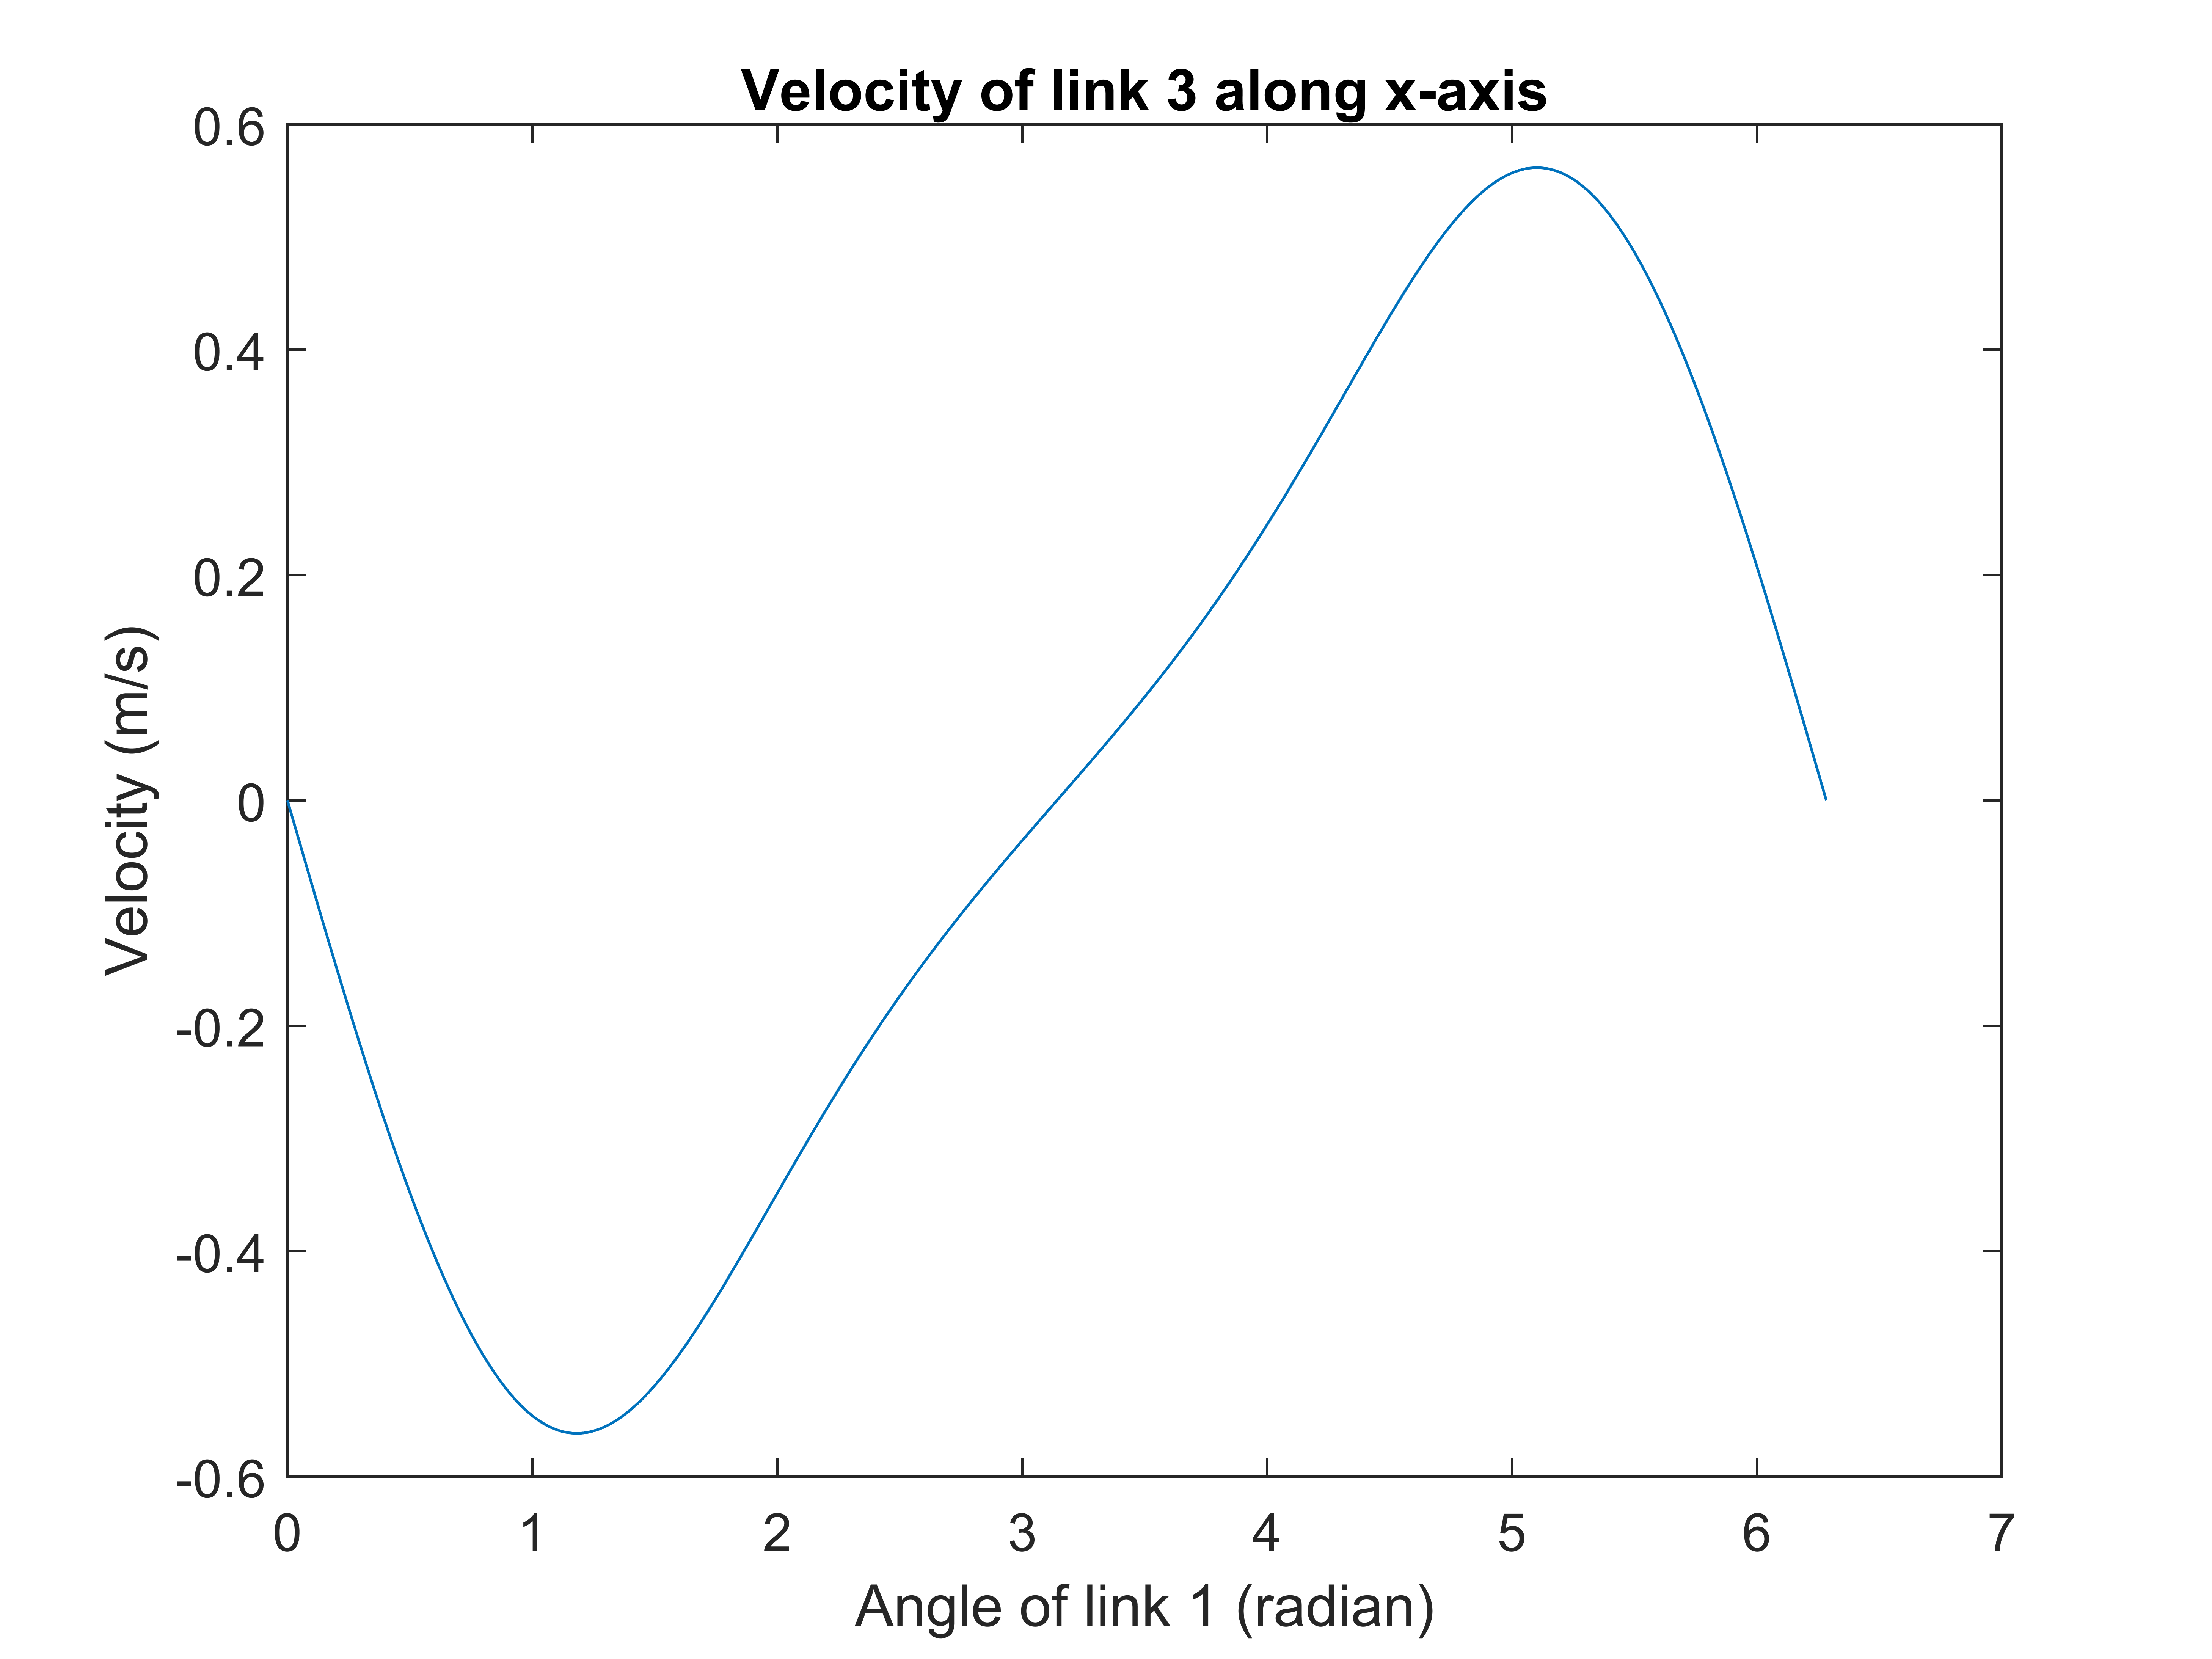
\includegraphics[width=60mm]{images/v_RRRT.png}
	\end{figure}
\end{minipage}\hfill
\begin{minipage}{0.5\linewidth}
	\begin{figure}
		\centering
		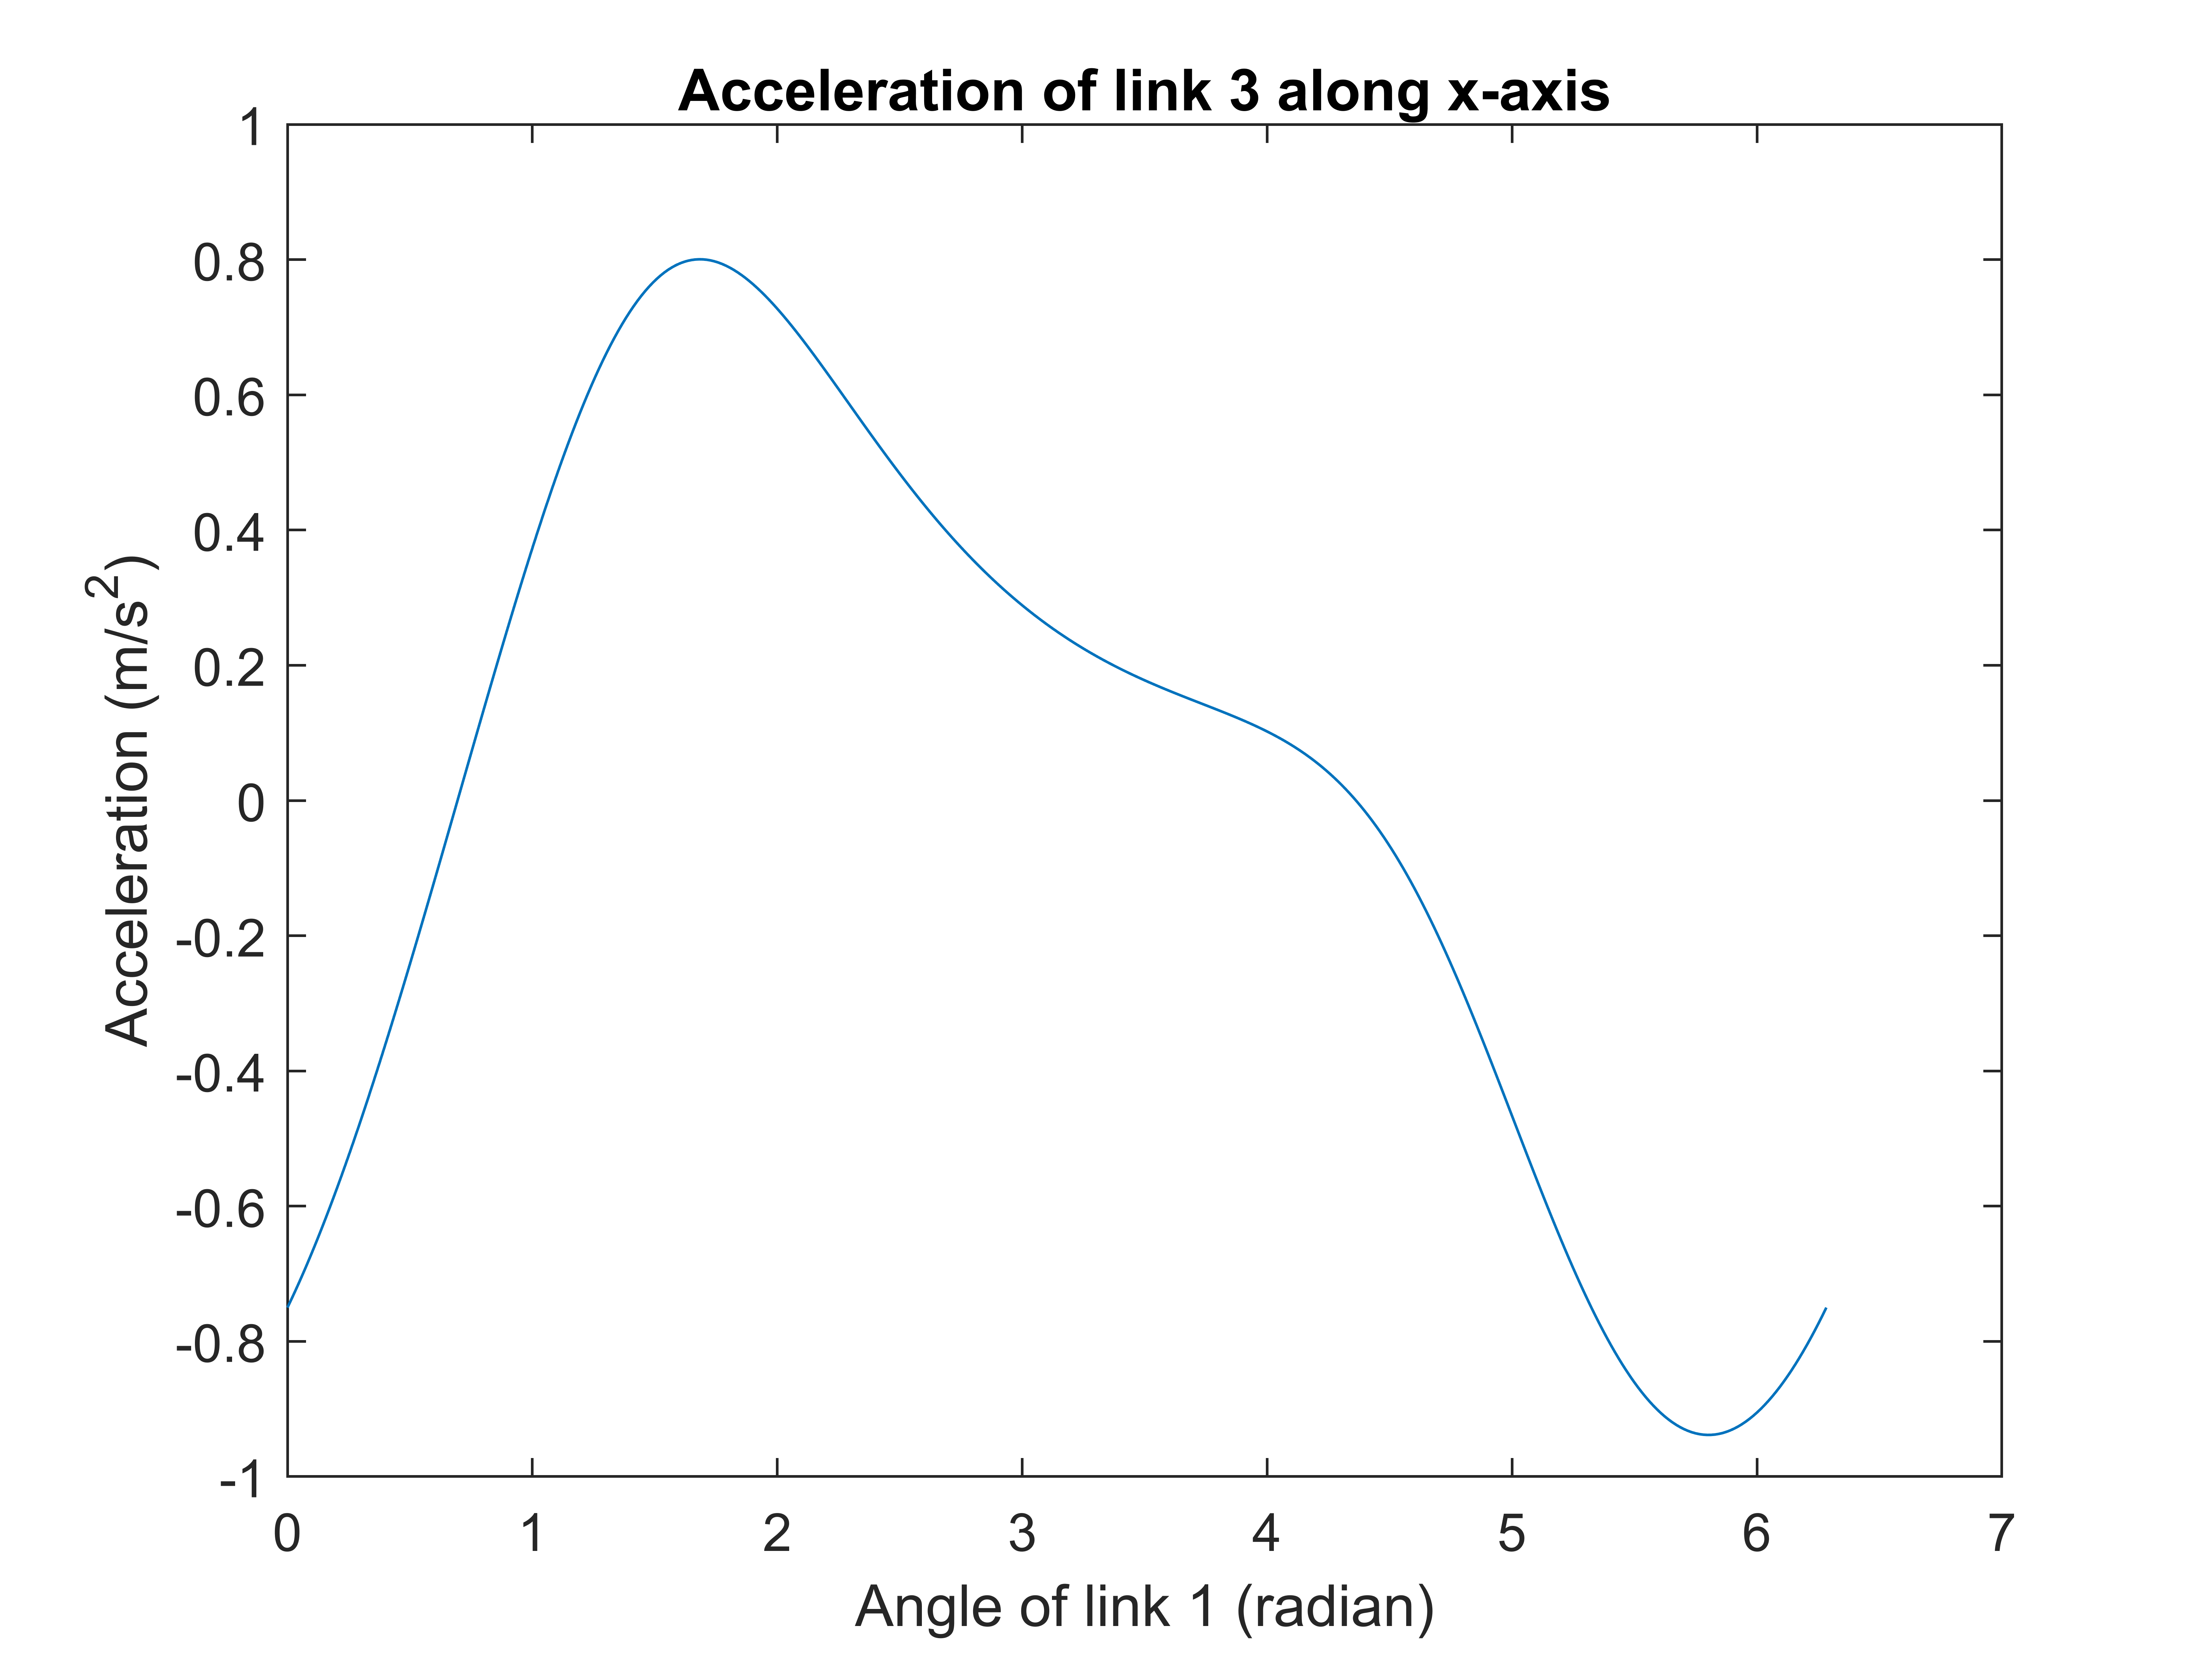
\includegraphics[width=60mm]{images/a_RRRT.png}
	\end{figure}
\end{minipage}
\end{table}
\end{frame}